\Section{parallel}{Parallel Haskell}

Parallel Haskell is all about making Haskell programs run
\emph{faster} by dividing the work to be done between multiple
processors.  Now that processor manufacturers have largely given up
trying to squeeze more performance out of individual processors and
have refocussed their attention on providing us with more processors
instead, the biggest gains in performance are to be had by using
parallel techniques in our programs so as to make use of these extra
cores.

We might wonder whether the compiler could automatically parallelise
programs for us.  After all, it should be easier to do this in a pure
functional language where the only dependencies between computations
are data dependencies, and those are mostly perspicuous and thus
readily analysed.  In contrast, when effects are unrestricted,
analysis of dependencies tends to be much harder, leading to greater
approximation and a large degree of false dependencies.  However, even
in a language with only data dependencies, automatic parallelisation
still suffers from an age-old problem: managing parallel tasks requires
some bookkeeping relative to sequential execution and thus has an
inherent overhead, so the size of the parallel tasks must be large
enough to overcome the overhead.  Analysing costs at compile time is
hard, so one approach is to use runtime profiling to find tasks that
are costly enough and can also be run in parallel, and feed this
information back into the compiler.  Even this, however, has not been
terribly successful in practice \cite{fdip}.

Fully automatic parallelisation is still a pipe dream.  However, the
parallel programming models provided by Haskell do succeed in
eliminating some mundane or error-prone aspects traditionally
associated with parallel programming:

\begin{itemize}
\item Parallel programming in Haskell is \emph{deterministic}: the
  parallel program always produces the same answer, regardless how
  many processors are used to run it, so parallel programs can be
  debugged without actually running them in parallel.

\item Parallel Haskell programs do not explicitly deal with
  \emph{synchronisation} or \emph{communication}.  Synchronisation is
  the act of waiting for other tasks to complete, perhaps due to data
  dependencies.  Communication involves the transmission of results
  between tasks running on different processors.  Synchronisation is
  handled automatically by the GHC runtime system and/or the
  parallelism libraries.  Communication is implicit in GHC since all
  tasks share the same heap, and can share objects without
  restriction.  In this setting, although there is no explicit
  communication at the program level or even the runtime level, at the
  hardware level communication re-emerges as the transmission of data
  between the caches of the different cores.  Excessive communication
  can cause contention for the main memory bus, and such overheads can
  be difficult to diagnose.
\end{itemize}

Parallel Haskell does require the programmer to think about
\textbf{Partitioning}.  The programmer's job is to subdivide the work
into tasks that can execute in parallel.  Ideally, we want to have
enough tasks that we can keep all the processors busy for the entire
runtime.  However, our efforts may be thwarted:
  \begin{itemize}
    \item \textbf{Granularity}.  If we make our tasks too small, then
      the overhead of managing the tasks outweighs any benefit we
      might get from running them in parallel.  So granularity should
      be large enough to dwarf the overheads, but not too large,
      because then we risk not having enough work to keep all the
      processors busy, especially towards the end of the execution
      when there are fewer tasks left.
    \item \textbf{Data dependencies} between tasks enforce
      sequentialisation.  GHC's two parallel programming models take
      different approaches to data dependencies: in \emph{Strategies}
      (\secref{strategies}), data dependencies are entirely implicit,
      whereas in the \emph{Par monad} (\secref{monad-par}), they are
      explicit.  This makes programming with Strategies somewhat more
      concise, at the expense of the possibility that hidden
      dependencies could cause sequentialisation at runtime.
  \end{itemize}


In this tutorial we will describe two parallel programming models
provided by GHC.  The first, \emph{Evaluation Strategies}
\cite{seq-no-more} (Strategies for short), is well-established and
there are many good examples of using Strategies to write parallel
Haskell programs.  The second is a dataflow programming model based
around a @Par@ monad \cite{monad-par}.  This is a newer programming
model in which it is possible to express parallel coordination more
explicitly than with Strategies, though at the expense of some of the
conciseness and modularity of Strategies.

\Subsection{par-eval}{Basic parallelism: the \texttt{Eval} monad}

In this section we will demonstrate how to use the basic parallelism
abstractions in Haskell to perform some computations in parallel.  As
a running example that you can actually test yourself, we use a Sudoku
solver\footnote{The Sudoku solver code can be found in the module
  @Sudoku.hs@ in the samples that accompany this tutorial.}.  The
Sudoku solver is very fast, and can solve all 49,000 of the known
puzzles with 17
clues\footnote{\url{http://mapleta.maths.uwa.edu.au/~gordon/sudokumin.php}}
in about 2 minutes.

We start with some ordinary sequential code to solve a set of Sudoku
problems read from a file:

\begin{haskell}
import Sudoku
import Control.Exception
import System.Environment

main :: IO ()
main = do
    [f] <- getArgs
    grids <- fmap lines $ readFile f
    mapM_ (evaluate . solve) grids
\end{haskell}

The module @Sudoku@ provides us with a function @solve@ with type

\begin{haskell}
solve :: String -> Maybe Grid
\end{haskell}

\noindent where the @String@ represents a single Sudoku problem, and
@Grid@ is a representation of the solution.  The function returns
@Nothing@ if the problem has no solution.  For the purposes of this
example we are not interested in the solution itself, so our @main@
function simply calls @evaluate . solve@ on each line of the file (the
file will contain one Sudoku problem per line).  The @evaluate@
function comes from @Control.Exception@ and has type

\begin{haskell}
evaluate :: a -> IO a
\end{haskell}

\noindent It evaluates its argument to \emph{weak-head normal form}.
Weak-head normal form just means that the expression is evaluated as
far as the first constructor; for example, if the expression is a
list, then @evaluate@ would perform enough evaluation to determine
whether the list is empty (@[]@) or non-empty (@_:_@), but it would
not evaluate the head or tail of the list.  The @evaluate@ function
returns its result in the @IO@ monad, so it is useful for forcing
evaluation at a particular time.

Compile the program as follows:

{\small \begin{verbatim}
$ ghc -O2 sudoku1.hs -rtsopts
[1 of 2] Compiling Sudoku           ( Sudoku.hs, Sudoku.o )
[2 of 2] Compiling Main             ( sudoku1.hs, sudoku1.o )
Linking sudoku1 ...
\end{verbatim}}

\noindent and run it on 1000 sample problems:

{\small \begin{verbatim}
$ ./sudoku1 sudoku17.1000.txt +RTS -s
./sudoku1 sudoku17.1000.txt +RTS -s 
   2,392,127,440 bytes allocated in the heap
      36,829,592 bytes copied during GC
         191,168 bytes maximum residency (11 sample(s))
          82,256 bytes maximum slop
               2 MB total memory in use

  Generation 0:  4570 collections, 0 parallel, 0.14s, 0.13s elapsed
  Generation 1:    11 collections, 0 parallel, 0.00s, 0.00s elapsed

  Parallel GC work balance: -nan (0 / 0, ideal 1)

                        MUT time (elapsed)       GC time  (elapsed)
  Task  0 (worker) :    0.00s    (  0.00s)       0.00s    (  0.00s)
  Task  1 (worker) :    0.00s    (  2.92s)       0.00s    (  0.00s)
  Task  2 (bound)  :    2.92s    (  2.92s)       0.14s    (  0.14s)

  SPARKS: 0 (0 converted, 0 pruned)

  INIT  time    0.00s  (  0.00s elapsed)
  MUT   time    2.92s  (  2.92s elapsed)
  GC    time    0.14s  (  0.14s elapsed)
  EXIT  time    0.00s  (  0.00s elapsed)
  Total time    3.06s  (  3.06s elapsed)

  %GC time       4.6%  (4.6% elapsed)

  Alloc rate    818,892,766 bytes per MUT second

  Productivity  95.4% of total user, 95.3% of total elapsed
\end{verbatim}}

\noindent The argument @+RTS -s@ instructs the GHC runtime system to
emit the statistics you see above. These are particularly helpful as a
first step in analysing parallel performance.  The output is explained
in detail in the GHC User's Guide, but for our purposes we are
interested in one particular metric: @Total time@.  This figure is
given in two forms: the first is the total CPU time used by the
program, and the second figure is the \emph{elapsed}, or wall-clock,
time.  Since we are running on a single processor, these times are
identical (sometimes the elapsed time might be slightly larger due to
other activity on the system).

This program should parallelise quite easily; after all, each problem
can be solved completely independently of the others.  First, we
will need some basic functionality for expressing parallelism, which
is provided by the module @Control.Parallel.Strategies@:

\begin{haskell}
data Eval a
instance Monad Eval

runEval :: Eval a -> a

rpar :: a -> Eval a
rseq :: a -> Eval a
\end{haskell}

\noindent Parallel coordination will be performed in a monad,
namely the @Eval@ monad.  The reason for this is that parallel
programming fundamentally involves \emph{ordering} things: start
evaluating @a@ in parallel, \emph{and then} evaluate @b@.  Monads are good
for expressing ordering relationships in a compositional way.

The @Eval@ monad provides a @runEval@ operation that lets us extract
the value from @Eval@.  Note that @runEval@ is completely pure -
there's no need to be in the @IO@ monad here.

The @Eval@ monad comes with two basic operations, @rpar@ and @rseq@.
The @rpar@ combinator is used for creating parallelism; it says ``my
argument could be evaluated in parallel'', while @rseq@ is used for
forcing sequential evaluation: it says ``evaluate my argument now''
(to weak-head normal form).  These two operations are typicaly used
together - for example, to evaluate @A@ and @B@ in parallel, we could
apply @rpar@ on @A@, followed by @rseq@ on @B@.

Returning to our Sudoku example, let us add some parallelism to make
use of two processors.  We have a list of problems to solve, so it
should suffice to divide the list in two and solve the problems in
each half of the list in parallel.  Here is some code to do just
that\footnote{full code in sample @sudoku2.hs@}:

\begin{numhaskell}
    let (as,bs) = splitAt (length grids `div` 2) grids

    evaluate $ runEval $ do
       a <- rpar (deep (map solve as))
       b <- rpar (deep (map solve bs))
       rseq a
       rseq b
       return ()
\end{numhaskell}

\noindent line 1 divides the list into two equal (or nearly-equal)
sub-lists, @as@ and @bs@.  The next part needs more explanation:

\begin{itemize}
\item[3] We are going to @evaluate@ an application of @runEval@
\item[4] Create a parallel task to compute the solutions to the
  problems in the sub-list @as@.  The expression @map solve as@
  represents the solutions; however, just evaluating this expression
  to weak-head normal form will not actually compute any of the
  solutions, since it will only evaluate as far as the first @(:)@
  cell of the list.  We need to fully evaluate the whole list,
  including the elements.  This is why we added an application of the
  @deep@ function, which is defined as follows:

\begin{haskell}
deep :: NFData a => a -> a
deep a = deepseq a a
\end{haskell}
\noindent @deep@ evaluates the entire structure of its argument
(reducing it to \emph{normal form}), before returning the argument
itself.  It is defined in terms of the function @deepseq@, which is
available from the @Control.DeepSeq@ module.

  Not evaluating deeply enough is a common mistake when using the
  @rpar@ monad, so it is a good idea to get into the habit of
  thinking, for each @rpar@, ``how much of this structure do I want to
  evaluate in the parallel task?'' (indeed, it is such a common
  problem that in the @Par@ monad to be introduced later, we went so
  far as to make @deepseq@ the default behaviour).

\item[5] Create a parallel task to compute the solutions to @bs@,
  exactly as for @as@.
\item[6-7] Using @rseq@, we wait for both parallel tasks to complete.
\item[8] Finally, return (for this example we aren't interested in the
  results themselves, only in the act of computing them).
\end{itemize}

In order to use parallelism with GHC, we have to add the @-threaded@
option, like so:

{\small \begin{verbatim}
$ ghc -O2 sudoku2.hs -rtsopts -threaded
[2 of 2] Compiling Main             ( sudoku2.hs, sudoku2.o )
Linking sudoku2 ...
\end{verbatim}}

\noindent Now, we can run the program using 2 processors:

{\small
\begin{verbatim}
$ ./sudoku2 sudoku17.1000.txt +RTS -N2 -s
./sudoku2 sudoku17.1000.txt +RTS -N2 -s 
   2,400,125,664 bytes allocated in the heap
      48,845,008 bytes copied during GC
       2,617,120 bytes maximum residency (7 sample(s))
         313,496 bytes maximum slop
               9 MB total memory in use

  Gen 0: 2975 collections, 2974 parallel, 1.04s, 0.15s elapsed
  Gen 1:    7 collections,    7 parallel, 0.05s, 0.02s elapsed

  Parallel GC work balance: 1.52 (6087267 / 3999565, ideal 2)

                        MUT time (elapsed)       GC time  (elapsed)
  Task  0 (worker) :    1.27s    (  1.80s)       0.69s    (  0.10s)
  Task  1 (worker) :    0.00s    (  1.80s)       0.00s    (  0.00s)
  Task  2 (bound)  :    0.88s    (  1.80s)       0.39s    (  0.07s)
  Task  3 (worker) :    0.05s    (  1.80s)       0.00s    (  0.00s)

  SPARKS: 2 (1 converted, 0 pruned)

  INIT  time    0.00s  (  0.00s elapsed)
  MUT   time    2.21s  (  1.80s elapsed)
  GC    time    1.08s  (  0.17s elapsed)
  EXIT  time    0.00s  (  0.00s elapsed)
  Total time    3.29s  (  1.97s elapsed)

  %GC time      32.9%  (8.8% elapsed)

  Alloc rate    1,087,049,866 bytes per MUT second

  Productivity  67.0% of total user, 111.9% of total elapsed
\end{verbatim}}

Note that the @Total time@ now shows a marked difference between the
CPU time (3.29s) and the elapsed time (1.97s).  Previously the elapsed
time was 3.06s, so we can calculate the \emph{speedup} on 2 processors
as $3.06/1.97 = 1.55$.  Speedups are always calculated as a ratio of
wall-clock times.  The CPU time is a helpful metric for telling us how
busy our processors are, but as you can see here, the CPU time when
running on multiple processors is often greater than the wall-clock
time for a single processor, so it would be misleading to calculate
the speedup as the ratio of CPU time to wall-clock time (1.67 here).

Why is the speedup only 1.55, and not 2?  In general there could be a
host of reasons for this, not all of which are under the control of
the Haskell programmer.  However, in this case the problem is partly
of our doing, and we can diagnose it using the ThreadScope tool.  To
profile the program using ThreadScope we need to first recompile it
with the @-eventlog@ flag, run it with @+RTS -ls@, and then invoke
ThreadScope on the generated @sudoku2.eventlog@ file:

{\small \begin{verbatim}
$ rm sudoku2; ghc -O2 sudoku2.hs -threaded -rtsopts -eventlog
[2 of 2] Compiling Main             ( sudoku2.hs, sudoku2.o )
Linking sudoku2 ...
$ ./sudoku2 sudoku17.1000.txt +RTS -N2 -ls
$ threadscope sudoku2.eventlog
\end{verbatim}}

\begin{figure}
\begin{center}
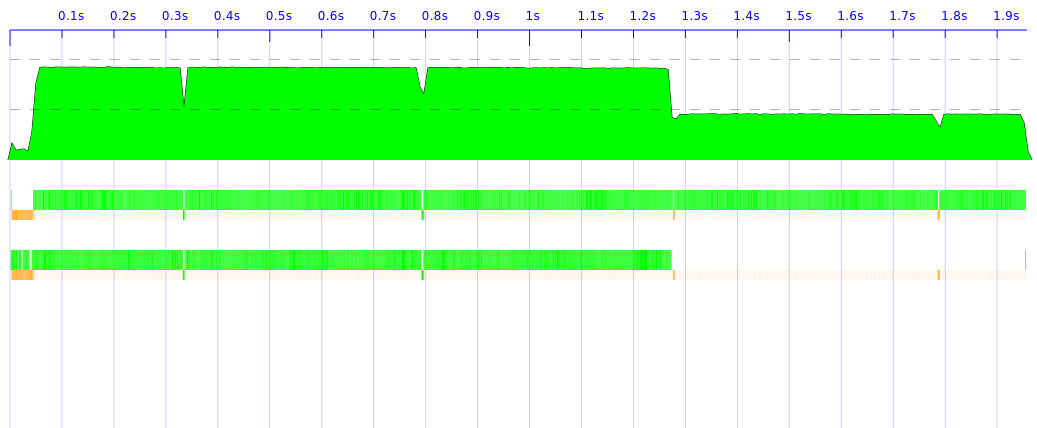
\includegraphics[scale=0.34]{sudoku2.png}
\end{center}
\caption{Sudoku2 ThreadScope profile}
\label{fig:sudoku2-threadscope}
\end{figure}

The ThreadScope profile is shown in \figref{sudoku2-threadscope}; this
graph was generated by selecting ``export to PNG'' from ThreadScope,
so it includes the timeline graph only, and not the rest of the
ThreadScope GUI.  The $x$ axis of the graph is time, and there are
three horizontal bars showing how the program executed over time.  The
topmost bar is known as the ``activity'' profile, and it shows how
many processors were executing Haskell code (as opposed to being idle
or garbage collecting) at a given point in time.  Underneath the
activity profile there is one bar per processor, showing what that
processor was doing at each point in the execution.  Each bar has two
parts:: the upper, thicker bar is green when that processor is
executing Haskell code, and the lower, narrower bar is orange or green
when that processor is performing garbage collection.\footnote{the
  distinction between orange and green during GC has to do with the
  kind of GC activity being performed, and need not concern us here.}

As we can see from the graph, there is a period at the end of the run
where just one processor is executing, and the other one is idle
(except for participating in regular garbage collections, which is
necessary for GHC's parallel garbage collector).  This indicates that
our two parallel tasks are uneven: one takes much longer to execute
than the other, and so we are not making full use of our 2 processors,
which results in less than perfect speedup.

Why should the workloads be uneven?  After all, we divided the list in
two, and we know the sample input has an even number of problems.  The
reason for the unevenness is that each problem does not take the same
amount of time to solve, it all depends on the searching strategy used
by the Sudoku solver\footnote{In fact, we ordered the problems in the
  sample input so as to clearly demonstrate the problem.}.  This
illustrates an important distinction between two partitioning
strategies:

\begin{itemize}
\item \textbf{Static Partitioning}, which is the technique we used to
  partition the Sudoku problems here, consists of dividing the work
  according to some pre-defined policy (here, dividing the list
  equally in two).

\item \textbf{Dynamic Partitioning} instead tries to distribute the
  work more evenly, by dividing the work into smaller tasks and only
  assigning tasks to processors when they are idle.
\end{itemize}

The GHC runtime system supports automatic distribution of the parallel
tasks; all we have to do to achieve dynamic partitioning is divide the
problem into small enough tasks and the runtime will do the rest for
us.

The argument to @rpar@ is called a \emph{spark}.  The runtime collects
sparks in a pool and uses this as a source of work to do when there
are spare processors available, using a technique called \emph{work
  stealing} \cite{multicore-ghc-09}.  Sparks may be evaluated at some
point in the future, or they might not --- it all depends on whether
there is spare processor capacity available.  Sparks are very cheap to
create (@rpar@ essentially just adds a reference to the expression to
an array).

So, let's try using dynamic partitioning with the Sudoku problem.
First we define an abstraction that will let us apply a function to a
list in parallel, @parMap@:

\begin{numhaskell}
parMap :: (a -> b) -> [a] -> Eval [b]
parMap f [] = return []
parMap f (a:as) = do
   b <- rpar (f a)
   bs <- parMap f as
   return (b:bs)
\end{numhaskell}

\noindent This is rather like a monadic version of @map@, except that
we have used @rpar@ to lift the application of the function @f@ to the
element @a@ into the @Eval@ monad.  Hence, @parMap@ runs down the
whole list, eagerly creating sparks for the application of @f@ to each
element, and finally returns the new list.  When @parMap@ returns, it
will have created one spark for each element of the list.

We still need to evaluate the result list itself, and that is
straightforward with @deep@:

\begin{haskell}
    evaluate $ deep $ runEval $ parMap solve grids
\end{haskell}

\noindent Running this new version\footnote{code sample @sudoku3.hs@}
yields more speedup:

{\small \begin{verbatim}
  Total time    3.55s  (  1.79s elapsed)
\end{verbatim}}

\noindent which we can calculate is equivalent to a speedup of
$3.06/1.79 = 1.7$, approaching the ideal speedup of 2.  Furthermore,
the GHC runtime system tells us how many sparks were created:

{\small \begin{verbatim}
  SPARKS: 1000 (1000 converted, 0 pruned)
\end{verbatim}}

\noindent we created exactly 1000 sparks, and they were all
\emph{converted} (that is, turned into real parallelism at runtime).
Sparks that are \emph{pruned} have been removed from the spark pool by
the runtime system, either because they were found to be already
evaluated, or because they were found to be not referenced by the rest
of the program, and so are deemed to be not useful.  We will discuss
the latter requirement in more detail in \secref{parlist}.

\begin{figure}
\begin{center}
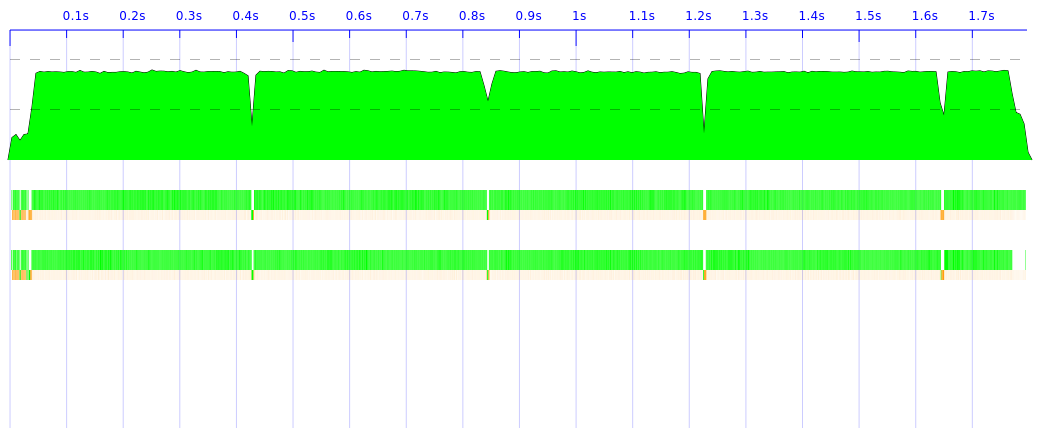
\includegraphics[scale=0.34]{sudoku3.png}
\end{center}
\caption{Sudoku3 ThreadScope profile}
\label{fig:sudoku3-threadscope}
\end{figure}

\begin{figure}
\begin{center}
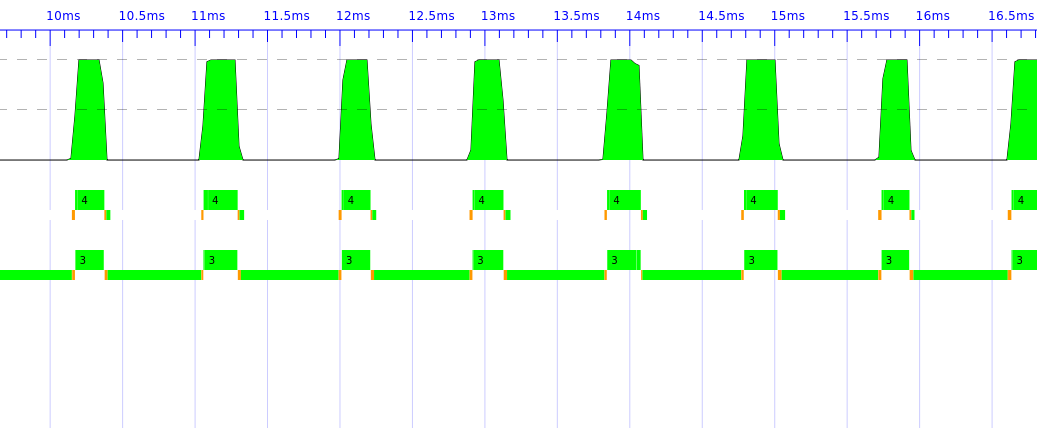
\includegraphics[scale=0.34]{sudoku3-zoom.png}
\end{center}
\caption{Sudoku3 (zoomed) ThreadScope profile}
\label{fig:sudoku3-zoom-threadscope}
\end{figure}

The ThreadScope profile looks much better
(\figref{sudoku3-threadscope}).  Furthermore, now that the runtime is
managing the work distribution for us, the program will automatically
scale to more processors.  On an 8 processor machine, for example:

{\small \begin{verbatim}
  Total time    4.46s  (  0.59s elapsed)
\end{verbatim}}

\noindent which equates to a speedup of 5.2 over the sequential
version.

If we look closely at the 2-processor profile there appears to be a
short section near the beginning where not much work is happening.  In
fact, zooming in on this section in ThreadScope
(\figref{sudoku3-zoom-threadscope}) reveals that both processors
are working, but most of the activity is garbage collection, and only
one processor is performing most of the garbage collection work.  In
fact, what we are seeing here is the program reading the input file
(lazily) and dividing it into lines, driven by the demand of @parMap@
which traverses the whole list of lines.

Since reading the file and dividing it into lines is a sequential
activity anyway, we could force it to happen all at once before we
start the main computation, by adding

\begin{haskell}
    evaluate (length grids)
\end{haskell}

\noindent (see code sample @sudoku4.hs@).  This makes no difference to
the overall runtime, but it divides the execution into sequential and
parallel parts, as we can see in ThreadScope
(\figref{sudoku4-threadscope}).

\begin{figure}
\begin{center}
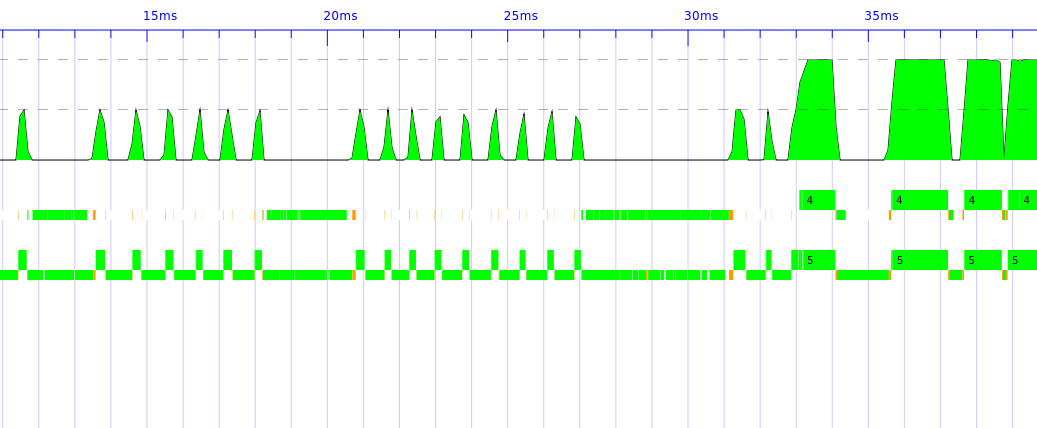
\includegraphics[scale=0.34]{sudoku4.png}
\end{center}
\caption{Sudoku4 ThreadScope profile}
\label{fig:sudoku4-threadscope}
\end{figure}

Now, we can read off the portion of the runtime that is sequential:
33ms.  When we have a sequential portion of our program, this affects
the maximum parallel speedup that is achievable, which we can
calculate using Amdahl's law.  Amdahl's law gives the maximum
achievable speedup as the ratio

\[
  \frac{1}{(1 - P) + \frac{P}{N}}
\]

\noindent where $P$ is the portion of the runtime that can be
parallelised, and $N$ is the number of processors available.  In our
case, $P$ is $(3.06-0.033)/3.06 = 0.9892$, and the maximum speedup is
hence 1.98.  The sequential fraction here is too small to make a
significant impact on the theoretical maximum speedup with 2
processors, but when we have more processors, say 64, it becomes much
more important: $1 / ((1-0.989) + 0.989/64) = 38.1$.  So no matter
what we do, this tiny sequential part of our program will limit the
maximum speedup we can obtain with 64 processors to 38.1.  In fact,
even with 1024 cores we could only achieve around 84 speedup, and it
is impossible to achieve a speedup of 91 no matter how many cores we
have.  Amdahl's law tells us that not only does parallel speedup
become harder to achieve the more processors we add, in practice most
programs have a theoretical maximum amount of parallelism.

\ToDo{Add something about Gustafson's law \url{http://en.wikipedia.org/wiki/Gustafson\%27s_Law}}

\Subsection{strategies}{Evaluation Strategies}

Evaluation Strategies \cite{trinder:strategies,seq-no-more} is an abstraction
layer built on top of the @Eval@ monad that allows larger parallel
specifications to be built in a compositional way.  Furthermore
Strategies allow parallel coordination to be described in a modular
way, separating parallelism from the algorithm to be parallelised.

A Strategy is merely a function in the @Eval@ monad that takes a value
of type @a@ and returns the same value:

\begin{haskell}
type Strategy a = a -> Eval a
\end{haskell}

\noindent Strategies are identity functions; that is, the value
returned by a @Strategy@ is observably equivalent to the value it was
passed.  Unfortunately the library cannot statically guarantee this
property for user-defined @Strategy@ functions, but it holds for the
@Strategy@ functions and combinators provided by the
@Control.Parallel.Strategies@ module.

We have already seen some simple Strategies, @rpar@ and @rseq@,
although we can now give their types in terms of @Strategy@:

\begin{haskell}
rseq :: Strategy a
rpar :: Strategy a
\end{haskell}

\noindent There are two further members of this family:

\begin{haskell}
r0 :: Strategy a
r0 x = return x

rdeepseq :: NFData a => Strategy a
rdeepseq x = rseq (deep x)
\end{haskell}

\noindent @r0@ is the @Strategy@ that evaluates nothing, and
@rdeepseq@ is the @Strategy@ that evaluates the entire structure of
its argument, which can be defined in terms of @deep@ that we saw
earlier.  Note that @rseq@ is necessary here: replacing @rseq@ with
@return@ would not perform the evaluation immediately, but would defer
it until the value returned by @rdeepseq@ is demanded (which might be
never).

We have some simple ways to build Strategies, but how is a Strategy
actually \emph{used}?  A @Strategy@ is just a function yielding a
computation in the @Eval@ monad, so we could use @runEval@.  For
example, applying the strategy @s@ to a value @x@ would be simply
@runEval (s x)@.  This is such a common pattern that the
Strategies library gives it a name, @using@:

\begin{haskell}
using :: a -> Strategy a -> a
x `using` s = runEval (s x)
\end{haskell}

\noindent @using@ takes a value of type @a@, a Strategy for @a@, and
applies the Strategy to the value.  The identity property for
@Strategy@ gives us that

{\small \begin{verbatim}
  x `using` s == x
\end{verbatim}}

\noindent which is a significant benefit of Strategies: every
occurrence of @`using` s@ can be deleted without affecting the
semantics.  Strictly speaking there are two caveats to this property.
Firstly, as mentioned earlier, user-defined @Strategy@ functions might
not satisfy the identity property.  Secondly, the expression @x `using` s@ might be
less defined than @x@, because it evaluates more structure of @x@ than
the context does.  So deleting @`using` s@ might have the effect of
making the program terminate with a result when it would previously
throw an exception or fail to terminate.  Making programs more defined
is generally considered to be a somewhat benign change in semantics
(indeed, GHC's optimiser can also make programs more defined under
certain conditions), but nevertheless it is a change in semantics.

\Subsubsection{parlist}{A Strategy for evaluating a list in parallel}

In \secref{par-eval} we defined a function @parMap@ that would map a
function over a list in parallel.  We can think of @parMap@ as a
composition of two parts:

\begin{itemize}
\item The algorithm: @map@
\item The parallelism: evaluating the elements of a list in parallel
\end{itemize}

\noindent and indeed with Strategies we can express it exactly this
way:

\begin{haskell}
parMap f xs = map f xs `using` parList rseq
\end{haskell}

\noindent The benefits of this approach are two-fold: not only does it
separate the algorithm from the parallelism, but it also \emph{reuses}
@map@, rather than re-implementing a parallel version.

The @parList@ function is a Strategy on lists, defined as follows:

\begin{haskell}
parList :: Strategy a -> Strategy [a]
parList strat []     = return []
parList strat (x:xs) = do
  x'  <- rpar (x `using` strat)
  xs' <- parList strat xs
  return (x':xs')
\end{haskell}

\noindent (in fact, @parList@ is already provided by
@Control.Parallel.Strategies@ so you don't have to define it yourself,
but we are using its implementation here as an illustration).

The @parList@ function is a \emph{parameterised} Strategy, that is, it
takes as an argument a Strategy on values of type @a@, and returns a
Strategy for lists of @a@.  This illustrates another important aspect
of Strategies: they are compositional, in the sense that we can build
larger strategies by composing smaller reusable components.  Here,
@parList@ describes a family of Strategies on lists that evaluate the
list elements in parallel.

On line 4, @parList@ calls @rpar@ to create a spark to evaluate the
current element of the list.  Note that the spark evaluates
@(x `using` strat)@: that is, it applies the argument Strategy @strat@ to
the list element @x@.

As @parList@ traverses the list sparking list elements, it remembers
each value returned by @rpar@ (bound to @x'@), and constructs a new
list from these values.  Why?  After all, this seems to be a lot of
trouble to go to, because it means that @parList@ is no longer
\emph{tail-recursive} --- the recursive call to @parList@ is not the
last operation in the @do@ on its right-hand side, and so @parList@
will require stack space linear in the length of the input list.

Couldn't we write a tail-recursive version instead?  For example:

\begin{haskell}
parList :: Strategy a -> Strategy [a]
parList strat xs = do go xs; return xs
  where go [] = return ()
        go (x:xs) = do
           rpar (x `using` strat)
           go xs
\end{haskell}

\noindent This typechecks, after all, and seems to call @rpar@ on each
list element as required.

\begin{figure}
\begin{center}
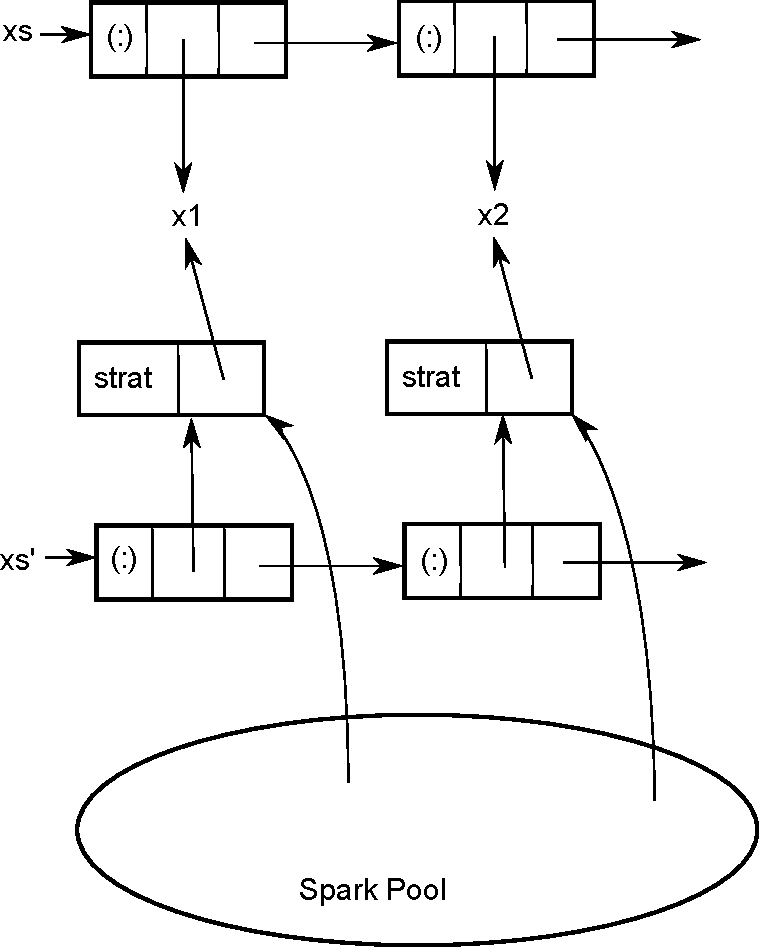
\includegraphics[scale=0.6]{parlist1.pdf}
\end{center}
\caption{\texttt{parList} heap structures}
\label{fig:parlist-heap}
\end{figure}

The difference is subtle but important, and is best understood via a
diagram (\figref{parlist-heap}).  At the top of the diagram we have
the input list @xs@: a linked list of cells, each of which points to a
list element (@x1@, @x2@, and so forth).  At the bottom of the diagram
is the \emph{spark pool}, the runtime system data structure that
stores references to sparks in the heap.  The other structures in the
diagram are built by @parList@ (the first version).  Each @strat@ box
represents @(x `using` strat)@ for an element @x@ of the original list, and @xs'@ is the linked list of cells in the output list.  The
spark pool contains pointers to each of the @strat@ boxes; these are
the pointers created by the @rpar@ calls.

Now, the spark pool only retains references to objects that are
required by the program.  If the runtime finds that the spark pool
contains a reference to an object that the program will never use,
then the reference is dropped, and any potential parallelism it
represented is lost.  This behaviour is a deliberate policy; if it
weren't this way, then the spark pool could retain data indefinitely,
causing a space leak (details can be found in \citet{seq-no-more}).

This is the reason for the list @xs'@.  Suppose we did not build the
new list @xs'@, as in the tail-recursive version of @parList@ above.
Then, the only reference to each @strat@ box in the heap would be from the
spark pool, and hence the runtime would automatically sweep all those
references from the spark pool, discarding the parallelism.  Hence we
build a new list @xs'@, so that the program can retain references to
the sparks for as long as it needs to.

This automatic discarding of unreferenced sparks has another benefit: suppose that under some
circumstances the program does not need the entire list.  If the
program simply forgets the unused remainder of the list, the runtime
system will clean up the unreferenced sparks from the spark pool, and
will not waste any further parallel processing resources on evaluating
those sparks.  The extra parallelism in this case is termed
\emph{speculative}, because it is not necessarily required, and the
runtime will automatically discard speculative tasks that it can prove
will never be required - a useful property!

While the runtime system's discarding of unreferenced sparks is
certainly useful in some cases, it can be tricky to work with, because
there is no language-level support for catching mistakes.  Fortunately
the runtime system will tell us if it garbage collects unreferenced
sparks; for example:

{\small \begin{verbatim}
  SPARKS: 144 (0 converted, 144 pruned)
\end{verbatim}}

\noindent A large number of sparks being ``pruned'' is a good
indication that sparks are being removed from the spark pool before
they can be used for parallelism.  Sparks can be pruned for several
reasons:

\begin{itemize}
\item The spark was a \emph{dud}: it was already evaluated at the
  point it was sparked.
\item The spark \emph{fizzled}: it was evaluated by some other thread
  before it could be evaluated in parallel.
\item The spark was garbage collected, as described above.
\end{itemize}

In fact, GHC from version 7.2.1 onwards separates these different
classifications in its output from @+RTS -s@:

{\small \begin{verbatim}
  SPARKS: 144 (0 converted, 0 dud, 144 GC'd, 0 fizzled)
\end{verbatim}}

\noindent Unless you are using speculation, then a non-zero figure for
GC'd sparks is probably a bad sign.

All of the combinators in the library @Control.Parallel.Strategies@
behave correctly with respect to retaining references to sparks when
necessary.  So the rules of thumb for not tripping up here are:

\begin{itemize}
\item Use @using@ to apply strategies: it encourages the right
  pattern, in which the program uses the results of applying the
  Strategy.
\item When writing your own @Eval@-monad code, remember to bind the
  result of @rpar@, and use its result.
\end{itemize}

\Subsubsection{using-parlist}{Using \texttt{parList}: the K-Means problem}

The @parList@ Strategy covers a wide range of uses for parallelism in
typical Haskell programs; in many cases, a single @parList@ is all
that is needed to expose sufficient parallelism.

Returning to our Sudoku solver from \secref{par-eval} for a moment,
instead of our own hand-written @parMap@, we could have used
@parList@:

\begin{haskell}
    evaluate $ deep $ map solve grids `using` parList rseq
\end{haskell}

\begin{figure}
\begin{center}
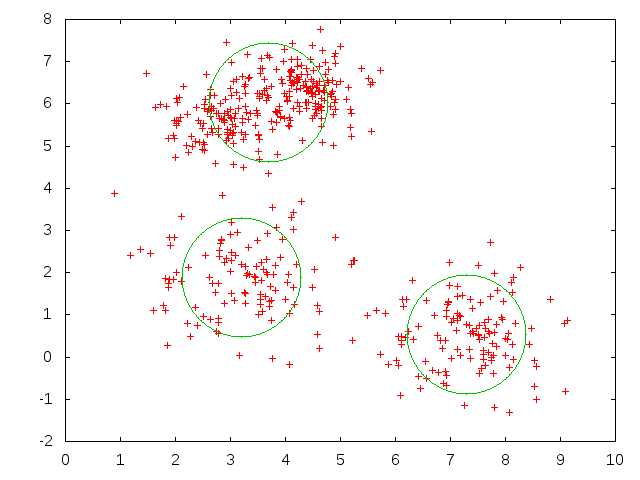
\includegraphics[scale=0.5]{kmeans-example.png}
\end{center}
\caption{The K-Means problem}
\label{fig:kmeans-example}
\end{figure}

Let's look at a slightly more involved example.  In the K-Means
problem, the goal is to partition a set of data points into clusters.
Finding an optimal solution to the problem is NP-hard, but there exist
several heuristic techniques that do not guarantee to find an optimal
solution, but work well in practice.  For example, given the data
points shown in \figref{kmeans-example}, the algorithm should discover
the clusters indicated by the circles.  Here we have only shown the
locations of the clusters, partitioning the points is achieved by
simply finding the closest cluster to each point.

The most well-known heuristic technique is Lloyd's algorithm, which
finds a solution by iteratively improving an initial guess, as
follows:

\begin{enumerate}
\item Pick an initial set of clusters by randomly assigning each point
  in the data set to a cluster.
\item Find the centroid of each cluster (the average of all the points
  in the cluster).
\item Assign each point to the cluster to which it is closest, this
  gives a new set of clusters.
\item Repeat steps 2--3 until the set of clusters stabilises.
\end{enumerate}

Of course the algorithm works in any number of dimensions, but we will
use 2 for ease of visualisation.

A complete Haskell implementation can be found in the directory
@kmeans@ in the sample code; \figref{kmeans-code} shows the core of
the algorithm.

\begin{figure}
\begin{numhaskell}
data Vector = Vector Double Double

addVector :: Vector -> Vector -> Vector
addVector (Vector a b) (Vector c d) = Vector (a+c) (b+d)

data Cluster = Cluster
               {
                  clId    :: !Int,
                  clCount :: !Int,
                  clSum   :: !Vector,
                  clCent  :: !Vector
               }

sqDistance :: Vector -> Vector -> Double
sqDistance (Vector x1 y1) (Vector x2 y2)
  = ((x1-x2)^2) + ((y1-y2)^2)

makeCluster :: Int -> [Vector] -> Cluster
makeCluster clid vecs
  = Cluster { clId = clid,
              clCount = count,
              clSum = vecsum,
              clCent = centre }
  where
   vecsum@(Vector a b)  = foldl' addVector (Vector 0 0) vecs
   centre = Vector (a / fromIntegral count)
                   (b / fromIntegral count)
   count = fromIntegral (length vecs)

-- assign each vector to the nearest cluster centre
assign :: Int -> [Cluster] -> [Vector] -> Array Int [Vector]
assign nclusters clusters points =
  accumArray (flip (:)) [] (0, nclusters-1)
     [ (clId (nearest p), p) | p <- points ]
  where
    nearest p = fst $ minimumBy (compare `on` snd)
                        [ (c, sqDistance (clCent c) p)
                        | c <- clusters ]

-- compute clusters from the assignment
makeNewClusters :: Array Int [Vector] -> [Cluster]
makeNewClusters arr =
  filter ((>0) . clCount) $
     [ makeCluster i ps | (i,ps) <- assocs arr ]

step :: Int -> [Cluster] -> [Vector] -> [Cluster]
step nclusters clusters points =
   makeNewClusters (assign nclusters clusters points)
\end{numhaskell}

\caption{Haskell code for K-Means}
\label{fig:kmeans-code}
\end{figure}

A data point is represented by the type @Vector@, which is just a pair
of @Double@s.  Clusters are represented by the type @Cluster@, which
contains its number, the count of points assigned to this cluster, the
sum of the @Vector@s in the cluster, and its centre.  Everything about
the cluster except its number is derivable from the set of points in
the cluster; this is expressed by the function @makeCluster@.
Essentially @Cluster@ caches various information about a cluster, and
the reason we need to cache these specific items will become clear
shortly.

The function @assign@ implements step 3 of the algorithm, assigning
points to clusters.  The @accumArray@ function is particularly useful
for this kind of bucket-sorting task.  The function @makeNewClusters@
implements step 2 of the algorithm, and finally @step@ combines
@assign@ and @makeNewClusters@ to implement one complete iteration.

To complete the algorithm we need a driver to repeatedly apply the @step@
function until convergence. The function @kmeans_seq@, in
\figref{kmeans_seq}, implements this.

\begin{figure}
\begin{haskell}
kmeans_seq :: Int -> [Vector] -> [Cluster] -> IO [Cluster]
kmeans_seq nclusters points clusters = do
  let
      loop :: Int -> [Cluster] -> IO [Cluster]
      loop n clusters | n > tooMany = return clusters
      loop n clusters = do
        hPrintf stderr "iteration %d\n" n
        hPutStr stderr (unlines (map show clusters))
        let clusters' = step nclusters clusters points
        if clusters' == clusters
           then return clusters
           else loop (n+1) clusters'
  --
  loop 0 clusters
\end{haskell}
\caption{Haskell code for kmeans\_seq}
\label{fig:kmeans_seq}
\end{figure}

How can this algorithm be parallelised?  One place that looks
straightforward to parallelise is the @assign@ function, since it is
essentially just a @map@ over the points.  However, that doesn't get
us very far: we cannot parallelise @accumArray@ directly, so we would
have to do multiple @accumArray@s and combine the results, and
combining elements would mean an extra list append.  The
@makeNewClusters@ operation parallelises easily, but only in so far as
each @makeCluster@ is independent of the others; typically the number
of clusters is much smaller than the number of points (e.g. a few
clusters to a few hundred thousand points), so we don't gain much
scalability by parallelising @makeNewClusters@.

We would like a way to parallelise the problem at a higher level.
That is, we would like to divide the set of points into chunks, and
process each chunk in parallel, somehow combining the results.  In
order to do this, we need a @combine@ function, such that

{\small \begin{verbatim}
 points == as ++ bs
   ==>
 step n cs points == step n cs as `combine` step n cs bs
\end{verbatim}}

Fortunately defining @combine@ is not difficult.  A cluster is a set
of points, from which we can compute a centroid.  The intermediate
values in this calcuation are the sum and the count of the data
points.  So a combined cluster can be computed from two independent
sub-clusters by taking the sum of these two intermediate values, and
re-computing the centroid from them.  Since addition is associative
and commutative, we can compute sub-clusters in any way we wish and
then combine them in this way.

Our Haskell code for combining two clusters is as follows:

\begin{haskell}
combineClusters c1 c2 =
  Cluster {clId = clId c1,
           clCount = count,
           clSum = vecsum,
           clCent = Vector (a / fromIntegral count)
                           (b / fromIntegral count)}
  where count = clCount c1 + clCount c2
        vecsum@(Vector a b)  = addVector (clSum c1) (clSum c2)
\end{haskell}

\noindent In general, however, we will be processing $N$ chunks of the
data space independently, each of which returns a set of clusters.  So
we need to reduce the $N$ sets of sets of clusters to a single set.
This is done with another @accumArray@:

\begin{haskell}
reduce :: Int -> [[Cluster]] -> [Cluster]
reduce nclusters css =
  concatMap combine $ elems $
    accumArray (flip (:)) [] (0,nclusters)
       [ (clId c, c) | c <- concat css]
 where
  combine [] = []
  combine (c:cs) = [foldr combineClusters c cs]
\end{haskell}

Now, the parallel K-Means implementation can be expressed as an
application of @parList@ to invoke @step@ on each chunk, followed by a
call to @reduce@ to combine the results from the chunks:

\begin{numhaskell}
kmeans_par :: Int -> Int -> [Vector] -> [Cluster]
           -> IO [Cluster]
kmeans_par chunks nclusters points clusters = do
  let chunks = split chunks points
  let
      loop :: Int -> [Cluster] -> IO [Cluster]
      loop n clusters | n > tooMany = return clusters
      loop n clusters = do
        hPrintf stderr "iteration %d\n" n
        hPutStr stderr (unlines (map show clusters))
        let
             new_clusterss =
                map (step nclusters clusters) chunks
                   `using` parList rdeepseq

             clusters' = reduce nclusters new_clusterss

        if clusters' == clusters
           then return clusters
           else loop (n+1) clusters'
  --
  loop 0 clusters
\end{numhaskell}

\noindent the only difference from the sequential implementation is at
lines 11--14, where we map @step@ over the chunks applying the
@parList@ strategy, and then call @reduce@.

Note that there's no reason the number of chunks has to be related to
the number of processors; as we saw earlier, it is better to produce
plenty of sparks and let the runtime schedule them automatically,
since this should enable the program to scale over a wide range of
processors.

\figref{kmeans-results} shows the speedups obtained by this
implementation for a randomly-generated data set consisting of 4
clusters with a total of approximately 170000 points in 2-D space.
The data was generated using the Haskell @normaldistribution@ package
in order to generate realistically clustered points\footnote{The
  program used to generate the data is provided as
  @kmeans/GenSamples.hs@ in the sample code distribution, and the
  sample data we used for this benchmark is provided in the files
  @kmeans/points.bin@ and @kmeans/clusters@ (the @GenSamples@ program
  will overwrite these files, so be careful if you run it!)}.  For this
benchmark we used 1000 for the @chunk@ parameter to @kmeans_par@.

The results show the algorithm scaling reasonably well up to 6 cores,
with a drop in performance at 8 cores.  We leave it as an exercise for
the reader to analyse the performance and improve it further!

\begin{figure}
\begin{center}
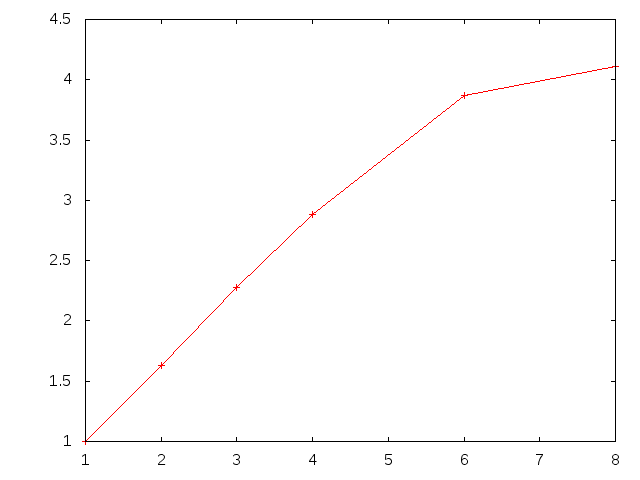
\includegraphics[scale=0.4]{kmeans-results.png}
\end{center}
\caption{Scaling of parallel K-Means}
\label{fig:kmeans-results}
\end{figure}

\Subsubsection{strat-further}{Further Reading}

We have barely scratched the surface of the possibilities with the
@Eval@ monad and Strategies here.  Topics that we have not covered
include:

\begin{itemize}
\item Sequential strategies, which allow greater control over the
  specification of \emph{evaluation degree} than is provided by @rseq@
  and @rdeepseq@.  See the documentation for the @Control.Seq@ module\footnote{\url{http://hackage.haskell.org/packages/archive/parallel/3.1.0.1/doc/html/Control-Seq.html}}.
\item Clustering, which allows greater control over granularity.
\item @parBuffer@: a combinator for parallelising lazy streams.
\end{itemize}

To learn more, we recommend the following resources:

\begin{itemize}
\item The documentation for the {\small @Control.Parallel.Strategies@} module\footnote{\url{http://hackage.haskell.org/packages/archive/parallel/3.1.0.1/doc/html/Control-Parallel-Strategies.html}}.
\item \citet{seq-no-more}, which explains the motivation behind the
  design and implementation of @Eval@ and Strategies.
\item \citet{pjsingh-tutorial}, an earlier tutorial covering
  basic parallelism in Haskell (beware: this dates from before the
  introduction of the @Eval@ monad).
\item \citet{trinder:strategies}, which has a wide range of examples.
  However beware: this paper is based on the earlier version of
  Strategies, and some of the examples may no longer work due to the
  new GC behaviour on sparks; also some of the names of functions and
  types in the library have since changed.
\end{itemize}

\Subsection{monad-par}{Dataflow parallelism: the \texttt{Par} monad}

Sometimes there is a need to be \emph{more explicit} about
dependencies and task boundaries than it is possible to be with @Eval@
and Strategies.  In these cases the usual recourse is to Concurrent
Haskell, where we can fork threads and be explicit about which thread
does the work.  However, that approach throws out the baby with the
bathwater: determinism is lost.  The programming model we introduce in
this section fills the gap between Strategies and Concurrent Haskell:
it is explicit about dependencies and task boundaries, but without
sacrificing determinism.  Furthermore the programming model has some
other interesting benefits: for example, it is implemented entirely as
a Haskell library and the implementation is readily modified to
accommodate alternative scheduling strategies.

As usual, the interface is based around a monad, this time called @Par@:

\begin{haskell}
  newtype Par a
  instance Functor Par
  instance Applicative Par
  instance Monad Par

  runPar :: Par a -> a
\end{haskell}

\noindent As with the @Eval@ monad, the @Par@ monad returns a pure
result.  However, use @runPar@ with care: internally it is much more
expensive than @runEval@, because (at least in the current
implementation) it will fire up a new scheduler instance consisting of
one worker thread per processor.  Generally speaking the program
should be using @runPar@ to schedule large-sale parallel tasks.

The purpose of @Par@ is to introduce parallelism, so we need a way to
create parallel tasks:

\begin{haskell}
  fork :: Par () -> Par ()
\end{haskell}

\noindent @fork@ does exactly what you would expect: the computation
passed as the argument to @fork@ (the ``child'') is executed
concurrently with the current computation (the ``parent'').

Of course, @fork@ on its own isn't very useful; we need a way to
communicate results from the child of @fork@ to the parent, or in
general between two parallel @Par@ computations.  Communication is
provided by the @IVar@ type\footnote{@IVar@ is so-called because it is an implementation of
I-Structures, a concept from the Parallel Haskell variant pH} and its operations:

\begin{haskell}
  data IVar a  -- instance Eq

  new :: Par (IVar a)
  put :: NFData a => IVar a -> a -> Par ()
  get :: IVar a -> Par a
\end{haskell}

\noindent @new@ creates a new @IVar@, which is initially empty; @put@
fills an @IVar@ with a value, and @get@ retrieves the value of an
@IVar@ (waiting until a value has been @put@ if necessary).  Multiple
@put@s to the same @IVar@ result in an error.

The @IVar@ type is a relative of the @MVar@ type that we shall see
later in the context of Concurrent Haskell (\secref{mvars}), the main
difference being that an @IVar@ can only be written once.  An @IVar@
is also like a \emph{future} or \emph{promise}, concepts that may be
familiar from other parallel or concurrent languages.

Together, @fork@ and @IVar@s allow the construction of
\emph{dataflow} networks.  The nodes of the network are created by
@fork@, and edges connect a @put@ with each @get@ on that @IVar@.  For
example, suppose we have the following four functions:

\begin{haskell}
f :: In -> A
g :: A -> B
h :: A -> C
j :: (B,C) -> Out
\end{haskell}

\noindent Composing these functions forms the following dataflow graph:

\begin{center}
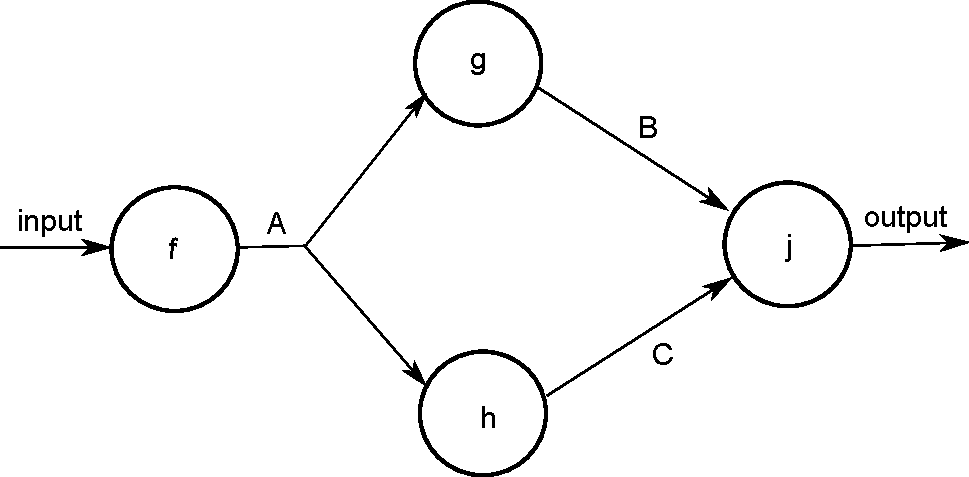
\includegraphics[scale=0.6]{dataflow.pdf}
\end{center}

There are no sequential dependencies between @g@ and @h@, so they
could run in parallel.  In order to take advantage of the parallelism
here, all we need to do is express the graph in the @Par@ monad:

\begin{haskell}
do
   [ia,ib,ic] <- replicateM 4 new

   fork $ do x <- get input
             put ia (f x)

   fork $ do a <- get ia
             put ib (g a)

   fork $ do a <- get ia
             put ic (h a)

   fork $ do b <- get ib
             c <- get ic
             put output (j b c)
\end{haskell}

\noindent For each edge in the graph we make an @IVar@ (here @ia@,
@ib@ and so on).  For each node in the graph we call @fork@, and the
code for each node calls @get@ on each input, and @put@ on each output
of the node.  The order of the @fork@ calls is irrelevant --- the
@Par@ monad will execute the graph, resolving the dependencies at
runtime.

While the @Par@ monad is particularly suited to expressing dataflow
networks, it can also express other common patterns too.  For example,
we can build an equivalent of the @parMap@ combinator that we saw
earlier in \secref{par-eval}.  First, we build a simple abstraction
for a parallel computation that returns a result:

\begin{haskell}
spawn :: NFData a => Par a -> Par (IVar a)
spawn p = do
  i <- new
  fork (do x <- p; put i x)
  return i
\end{haskell}

\noindent The @spawn@ function forks a computation in parallel, and
returns an @IVar@ that can be used to wait for the result.

Now, parallel map consists of calling @spawn@ to apply the function to
each element of the list, and then waiting for all the results:

\begin{haskell}
parMapM :: NFData b => (a -> Par b) -> [a] -> Par [b]
parMapM f as = do
  ibs <- mapM (spawn . f) as
  mapM get ibs
\end{haskell}

\noindent Note that there are a couple of differences between this and
the @Eval@ monad @parMap@.  First, the function argument returns its
result in the @Par@ monad; of course it is easy to lift an arbitrary
pure function to this type, but the monadic version allows the
computation on each element to produce more parallel tasks, or augment
the dataflow graph in other ways.  Second, @parMapM@ waits for all the
results.  Depending on the context, this may or may not be the most
useful behaviour, but of course it is easy to define the other version
if necessary.

\Subsubsection{monad-par-infer}{A parallel type inferencer}

In this section we will parallelise a type inference engine using the
@Par@ monad.  Type inference is a natural fit for the dataflow model,
because we can consider each binding to be a node in the graph, and
the edges of the graph carry inferred types from bindings to usage
sites in the program.

For example, consider the following set of bindings that we
want to infer types for:

{\small \begin{verbatim}
  f = ...
  g = ... f ...
  h = ... f ...
  j = ... g ... h ...
\end{verbatim}}

This pattern gives rise to a dataflow graph with exactly the shape of
the example 4-node graph in the previous section: after we have
inferred a type for @f@, we can use that type to infer types for @g@
and @h@ (in parallel), and once we have the types for @g@ and @h@ we
can infer a type for @j@.

Building a dataflow graph for the type inference problem allows the
maximum amount of parallelism to be extracted from the type inference
process.  The actual amount of parallelism present depends on the
structure of the input program, however.

The parallel type inferencer can be found in the directory @parinfer@
of the code samples, and is derived from a (rather ancient) type
inference engine written by Phil Wadler.  The types from the inference
engine that we will need to work with are as follows:

\begin{numhaskell}
type VarId = String -- variables

data Env -- environment for the type inferencer

-- build environments
makeEnv :: [(VarId,Type)] -> Env

data MonoType -- monomorphic types
data PolyType -- polymorphic types

-- Terms in the input program
data Term = Let VarId Term Term | ...
\end{numhaskell}

The input to this type inferencer is a single @Term@ which may contain
@let@ bindings, and so to parallelise it we will strip off the outer
@let@ bindings and typecheck them in parallel.  The inner term will be
typechecked using the ordinary sequential inference engine.  We could
have a more general parallel type inference algorithm by always
typechecking a @let@ binding in parallel with the body, rather than
just for the outer @let@s, but that would require threading the @Par@
monad through the type inference engine, so for this simple example we
are only parallelising inference for the outer bindings.

We need two functions from the inference engine.  First, a way to
infer a polymorphic type for the right-hand side of a binding:

\begin{haskell}
inferTopRhs :: Env -> Term -> PolyType
\end{haskell}

\noindent and secondly, a way to run the inference engine on an
arbitrary term:

\begin{haskell}
inferTopTerm :: Env -> Term -> MonoType
\end{haskell}

The basic idea is that while the sequential inference engine uses an
@Env@ that maps @VarId@s to @PolyType@s, the parallel part of the
inference engine will use an environment that maps @VarId@s to
@IVar PolyType@, so that we can @fork@ the inference engine for a
given binding, and then wait for its result later\footnote{We are
  ignoring the possibility of type errors here; in a real
  implementation the @IVar@ would probably contain an @Either@ type
  representing either the inferred type or an error.}.  The environment
for the parallel type inferencer is called @TopEnv@:

\begin{haskell}
type TopEnv = Map VarId (IVar PolyType)
\end{haskell}

All that remains is to write the top-level loop.  We will write a
function @inferTop@ with the following type:

\begin{haskell}
inferTop :: TopEnv -> Term -> Par MonoType
\end{haskell}

\noindent There are two cases to consider.  First, when we are looking at a
@let@ binding:

\begin{numhaskell}
inferTop topenv (Let x u v) = do
    vu <- new

    fork $ do
      let fu = Set.toList (freeVars u)
      tfu <- mapM (get . fromJust . flip Map.lookup topenv) fu
      let aa = makeEnv (zip fu tfu)
      put vu (inferTopRhs aa u)

    inferTop (Map.insert x vu topenv) v
\end{numhaskell}

\noindent On line 2 we create a new @IVar@ @vu@ to hold the type of @x@.  Lines
4--8 implement the typechecking for the binding:

\begin{itemize}
\item [4] We @fork@ here, so that the binding is typechecked in
  parallel,
\item [5] Find the @IVar@s corresponding to the free variables of the right-hand side
\item [6] Call @get@ for each of these, thus waiting for the
  typechecking of the binding corresponding to each free variable
\item [7] Make a new @Env@ with the types we obtained on line 6
\item [8] Call the type inferencer for the right-hand side, and put the
  result in the @IVar@ @vu@.
\end{itemize}

The main computation continues (line 10) by typechecking the body of
the @let@ in an environment in which the bound variable @x@ is mapped
to the @IVar@ @vu@.

The other case of @inferTop@ handles all other expression constructs:

\begin{numhaskell}
inferTop topenv t = do
    let (vs,ivs) = unzip (Map.toList topenv)
    tvs <- mapM get ivs
    let aa = makeEnv (zip vs tvs)
    return (inferTopTerm aa t)
\end{numhaskell}

\noindent This case is straightforward: just call @get@ to obtain the
inferred type for each binding in the @TopEnv@, construct an
@Env@, and call the sequential inferencer on the term @t@.

This parallel implementation works quite nicely.  For example, we have
constructed a synthetic input for the type checker, a fragment of
which is given below (the full version is in the file
@code/parinfer/example.in@).  The expression defines two sequences of
bindings which can be inferred in parallel.  The first sequence is the
set of bindings for @x@ (each successive binding for @x@ shadows the
previous), and the second sequence is the set of bindings for @y@.
Each binding for @x@ depends on the previous one, and similarly for
the @y@ bindings, but the @x@ bindings are completely independent of
the @y@ bindings.  This means that our parallel typechecking algorithm
should automatically infer types for the @x@ bindings in parallel with
the inference of the @y@ bindings, giving a maximum speedup of 2.

{\small \begin{verbatim}
let id = \x.x in
    let x = \f.f id id in
    let x = \f . f x x in
    let x = \f . f x x in
    let x = \f . f x x in
    ...
    let x = let f = \g . g x in \x . x in
    let y = \f.f id id in
    let y = \f . f y y in
    let y = \f . f y y in
    let y = \f . f y y in
    ...
    let y = let f = \g . g y in \x . x in
    \f. let g = \a. a x y in f
\end{verbatim}}

\noindent When we type check this expression with one processor, we
obtain the following result:

{\small \begin{verbatim}
$ ./infer <./example.in +RTS -s
  ...
  Total time    1.13s  (  1.12s elapsed)
\end{verbatim}}

\noindent and with two processors:

{\small \begin{verbatim}
$ ./infer <./example.in +RTS -s -N2
  ,..
  Total time    1.19s  (  0.60s elapsed)
\end{verbatim}}

\noindent representing a speedup of 1.87.

\Subsubsection{monad-par-reflections}{The \texttt{Par} monad compared
  to Strategies}

We have presented two different parallel programming models, each with
advantages and disadvantages.  Below we summarise the trade-offs so
that you can make an informed decision for a given task as to which is
likely to be the best choice:

\begin{itemize}
\item Using Strategies and the @Eval@ monad requires some
  understanding of the workings of lazy evaluation.  Newcomers often
  find this hard, and diagnosing problems can be difficult.  This is
  part of the motivation for the @Par@ monad: it makes all
  dependencies explicit, effectively replacing lazy evaluation with
  explicit @put@/@get@ on @IVar@s.  While this is certainly more
  verbose, it is less fragile and easier to work with.

  Programming with @rpar@ requires being careful about retaining
  references to sparks to avoid them being garbage collected; this can
  be subtle and hard to get right in some cases.  The @Par@ monad has
  no such requirements, although it does not support speculative
  parallelism in the sense that @rpar@ does: speculative paralelism
  in the @Par@ monad is always executed.

\item Strategies allow a separation between algorithm and parallelism,
  which allows more reuse in some cases.

\item The @Par@ monad requires threading the monad throughout a
  computation which is to be parallelised.  For example, to
  parallelise the type inference of all @let@ bindings in the example
  above would have required threading the @Par@ monad through the
  inference engine (or adding @Par@ to the existing monad stack),
  which might be impractical.  @Par@ is good for localised
  parallelism, whereas Strategies can be more easily used in cases
  that require parallelism in multiple parts of the program.

\item The @Par@ monad has more overhead than the @Eval@ monad,
  although there is no requirement to rebuild data structures as in
  @Eval@.  At the present time, @Eval@ tends to perform better at
  finer granularities, due to the direct runtime system support for
  sparks.  At larger granularities, @Par@ and @Eval@ perform
  approximately the same.

\item The @Par@ monad is implemented entirely in a Haskell library
  (the @monad-par@ package), and is thus readily modified should you
  need to.
\end{itemize}

% ToDo:
% \Subsection{skeletons}{Skeletons}

% ToDo:
% \Subsubsection{par-further}{Further reading}

